\documentclass[conference, a4paper]{IEEEtran}

% --- Recommended Packages ---
\usepackage{cite}
\usepackage{amsmath,amssymb,amsfonts}
\usepackage{algorithm}    % floating algorithm environment
\usepackage{algorithmic}  % \begin{algorithmic} content commands
\usepackage{graphicx}
\usepackage{textcomp}
\usepackage{xcolor}
\usepackage{booktabs}

\begin{document}

% --- Paper Title ---
\title{Performance Evaluation of xApp-based PRB Allocation in an O-RAN IAB Testbed}

% --- Author Block ---
\author{
    \IEEEauthorblockN{1\textsuperscript{st} Hsin-Jung Hsieh}
    \IEEEauthorblockA{\textit{Department of Electronic Engineering} \\
    \textit{National Taipei University of Technology}\\
    Taipei, Taiwan \\
    yt160533@gmail.com}
    \and
    \IEEEauthorblockN{2\textsuperscript{nd} Meng-Shiuan Pan}
    \IEEEauthorblockA{\textit{Department of Electronic Engineering} \\
    \textit{National Taipei University of Technology}\\
    Taipei, Taiwan \\
    mspan@ntut.edu.tw}
}

\maketitle

% --- Abstract ---
\begin{abstract}
This paper presents an experimental study of Physical Resource Block (PRB) allocation in a multi-hop Open Radio Access Network (O-RAN) Integrated Access and Backhaul (IAB) system. To address the high deployment cost of fiber-based backhaul and the implementation complexity of relay protocols, we build a practical IAB testbed using OpenAirInterface (OAI), Universal Software Radio Peripherals (USRPs), and Ubuntu hosts with low-latency kernels. Instead of relying on the full 3GPP Backhaul Adaptation Protocol (BAP), the proposed platform adopts a lightweight BAP-less design based on Linux IP forwarding and static routing. On top of this platform, we integrate a near-Real-Time Radio Intelligent Controller (near-RT RIC) and implement an xApp that adjusts the PRB split between backhaul and access links. We then compare fixed allocation ratios, such as 50/50, 30/70, and 10/90, together with an adaptive policy and the default proportional fair (PF) scheduler, and analyze their impact on end-to-end throughput and latency under realistic SDR constraints. The results show that different PRB allocation methods lead to different throughput-latency trade-offs across network conditions, and that the proposed platform is suitable for experimentally characterizing these scheduling behaviors rather than claiming that xApp-based control universally outperforms either fixed-ratio allocation or PF scheduling.
\end{abstract}

% --- Keywords ---
\begin{IEEEkeywords}
O-RAN, Integrated Access and Backhaul (IAB), PRB Allocation, xApp, near-RT RIC, OpenAirInterface, Testbed
\end{IEEEkeywords}

% --- Section I: Introduction ---
\section{Introduction}
The rapid densification of 5G networks has intensified the need to expand coverage and capacity without incurring a proportional increase in deployment cost. In practice, provisioning fiber backhaul for every small cell remains both costly and time-consuming, particularly in dense urban areas, temporary venues, and geographically constrained environments. Integrated Access and Backhaul (IAB) has emerged as a promising solution to this challenge by enabling the same radio infrastructure and spectrum resources to support both user access and wireless backhaul, thereby reducing fiber dependence while preserving deployment flexibility \cite{polese2020iab,ronkainen2021iab,3gpp38874}.

At the same time, the Open Radio Access Network (O-RAN) paradigm has introduced a more open and programmable framework for radio control. By disaggregating hardware and software and standardizing key interfaces, O-RAN allows operators to deploy intelligent control functions across multivendor platforms. In particular, the Radio Intelligent Controller (RIC) provides a practical mechanism for monitoring network conditions and enforcing near-real-time optimization through xApps \cite{polese2023coloran,villa2024x5g,cheng2024oranslice,oran-wg3-e2}.

However, the combination of multi-hop IAB and O-RAN also creates a challenging resource-allocation problem. In relay-based topologies, Physical Resource Blocks (PRBs) must be partitioned between backhaul and access links. When traffic demand varies across hops, a fixed or poorly matched PRB split can lead to persistent bottlenecks, queue buildup at intermediate nodes, and degraded end-to-end Quality of Service (QoS). This issue becomes even more pronounced in real SDR deployments, where scheduling latency, software processing overhead, and implementation-specific queue dynamics all affect measured performance.

In this paper, we address the gap between simulation-oriented IAB research and practical O-RAN implementation. We develop a multi-hop O-RAN IAB testbed based on OpenAirInterface (OAI) \cite{kaltenberger2021oai} and FlexRIC \cite{lacava2023flexric}, replace the heavyweight Backhaul Adaptation Protocol (BAP) data path with native Linux routing, and deploy an xApp on a near-RT RIC to control PRB allocation in real time. Rather than arguing that a customized policy should always outperform the default proportional fair (PF) scheduler, we use this platform to compare multiple PRB allocation methods and to characterize how different allocation strategies shape bottlenecks, throughput, and latency in a physical test environment.

The main contributions of this paper are summarized as follows:
\begin{itemize}
    \item We build a real multi-hop O-RAN IAB testbed using OAI, USRP hardware, and Ubuntu PREEMPT\_RT hosts, and we demonstrate a practical BAP-less forwarding architecture for SDR-based relay deployment.
    \item We design and integrate a custom xApp on a near-RT RIC to configure and evaluate multiple MAC-layer PRB allocation methods between backhaul and access links, including fixed-ratio and adaptive policies.
    \item We validate the proposed architecture with experimental measurements and show how different PRB splits lead to different throughput-latency trade-offs, which can then be compared against the default proportional fair (PF) scheduler.
\end{itemize}

% --- Section II: Related Work ---
\section{Related Work}
Integrated Access and Backhaul has been extensively studied as a cost-effective approach to extending 5G coverage without requiring fiber connectivity at every small cell. Early studies primarily focused on the architectural feasibility, protocol implications, and deployment potential of IAB, particularly in dense mmWave settings where access and backhaul must share spectrum efficiently \cite{polese2020iab,ronkainen2021iab}. These foundational works established the importance of jointly considering access and backhaul resources, but they mainly emphasized system architecture, standardization, and simulation-based performance characterization.

Subsequent research has examined resource allocation and routing in IAB networks in greater detail. Representative studies include semi-centralized resource management for 5G NR IAB and decentralized joint resource allocation and path selection for multi-hop topologies \cite{pagin2022semicentralized,alghafari2022decentralized}. In this line of work, the balance between backhaul and access resources is typically formulated as a throughput maximization, fairness optimization, or routing-scheduling co-design problem under half-duplex and bandwidth constraints. Although these studies provide valuable design insight, their evaluations are still predominantly based on analytical models or simulations, leaving implementation-level constraints largely abstracted away.

In parallel, O-RAN has enabled a programmable control framework through the near-RT RIC and xApps. Prior studies have shown that O-RAN can support closed-loop control, AI-driven decision making, and service-aware slicing on open experimental platforms, as illustrated by systems such as ColO-RAN, X5G, and ORANSlice \cite{polese2023coloran,villa2024x5g,cheng2024oranslice}. These efforts are important because they demonstrate practical integration across O-RAN software components, OpenAirInterface-based stacks, and programmable control loops. However, most of them focus on general O-RAN experimentation, traffic steering, or slicing, rather than on the specific multi-hop bottlenecks that arise when IAB nodes must divide radio resources between upstream backhaul and downstream access.

Accordingly, the key gap in the literature is not the lack of IAB allocation algorithms, but the lack of empirical comparison on an open, programmable, multi-hop O-RAN IAB platform. Our work addresses this gap by combining OpenAirInterface, Docker Compose-based multi-host deployment, a BAP-less Linux routing design, and near-RT RIC/xApp control in a real SDR testbed. Rather than claiming that a single handcrafted strategy is universally optimal, we experimentally compare fixed-ratio PRB allocation, an adaptive xApp policy, and the default PF scheduler to reveal their throughput-latency trade-offs in practical IAB operation.

% --- Section III: System Model ---
\section{System Model and Problem Formulation}
In this section, we define the mathematical model for our multi-hop O-RAN environment and formulate the PRB allocation problem.

\subsection{Network Architecture Model}
Consider a tree-topology O-RAN IAB network composed of a 5G Core, a Donor Central Unit (CU), a Donor Distributed Unit (DU), a set of IAB nodes $\mathcal{K} = \{1,2,\ldots,K\}$, and a set of served User Equipments (UEs) $\mathcal{U} = \{1,2,\ldots,U\}$. Some IAB nodes operate as relay nodes, whereas others operate as access IAB nodes that serve downstream UEs. Let the total system bandwidth be divided into a set of Physical Resource Blocks $\mathcal{N}_{PRB} = \{1,2,\ldots,N\}$.

Because the IAB nodes share radio resources between upstream backhaul and downstream access transmission, each node must partition the available PRBs across these two functions. Under half-duplex and finite-buffer constraints, over-provisioning one side of the link pair can starve the other side and cause queue imbalance across hops.

\subsection{Channel Model and Capacity}
The Signal-to-Interference-plus-Noise Ratio (SINR) for a link between node $i$ and node $j$ on PRB $n$ is given by:
\begin{equation}
    \gamma_{i,j}^n = \frac{P_{i}^n |h_{i,j}^n|^2}{I_{i,j}^n + \sigma^2}
\end{equation}
where $P_{i}^n$ is the transmit power, $h_{i,j}^n$ is the channel gain, $I_{i,j}^n$ represents the interference from other transmitting nodes, and $\sigma^2$ is the additive white Gaussian noise (AWGN) variance.

The achievable data rate for the link over PRB $n$ can be calculated using the Shannon capacity formula:
\begin{equation}
    R_{i,j}^n = W_{PRB} \log_2(1 + \gamma_{i,j}^n)
\end{equation}
where $W_{PRB}$ is the bandwidth of a single PRB. The total throughput of a specific link is the sum of the rates over all allocated PRBs.

\subsection{Problem Formulation}
Our objective is to study how PRB allocation affects end-to-end service throughput and relay congestion while maintaining feasible flow transfer through the relay chain. Let $x_{i,j}^n \in \{0, 1\}$ denote whether PRB $n$ is assigned to the link between nodes $i$ and $j$. A reference optimization objective can be written as:
\begin{align}
    \max_{\mathbf{x}} \quad & \sum_{u \in \mathcal{U}} \sum_{n \in \mathcal{N}_{PRB}} R_{k(u),u}^n x_{k(u),u}^n \\
    \textrm{s.t.} \quad & \sum_{i,j} x_{i,j}^n \le 1, \quad \forall n \in \mathcal{N}_{PRB} \label{eq:constraint_prb} \\
    & R_{donor, k} \ge \sum_{u \in \mathcal{U}_k} R_{k, u}, \quad \forall k \in \mathcal{K} \label{eq:constraint_flow}
\end{align}
where $k(u)$ denotes the serving IAB access node of UE $u$. Constraint \eqref{eq:constraint_prb} ensures that each PRB is assigned to at most one link simultaneously within the same cell; spatial reuse across non-interfering cells is abstracted away in this formulation, consistent with our single-donor, tree-topology testbed where each access DU operates on an isolated RF simulation channel. Constraint \eqref{eq:constraint_flow} represents flow conservation at the IAB node, ensuring that the backhaul capacity is sufficient to support the aggregated access traffic, thereby preventing bottleneck congestion.

In practice, our xApp is used as an experimental control mechanism rather than a guaranteed optimal solver. It can enforce predetermined PRB ratios and can also adapt the ratio according to the queue states of the donor-side backhaul and IAB-side access links. This design is intentionally lightweight so that it can operate within the timing constraints of the near-RT RIC and the SDR-based OAI stack while enabling fair comparison among several allocation methods.

% --- Section IV: Testbed Architecture ---
\section{Proposed IAB Testbed Architecture}
To evaluate the PRB allocation schemes, we construct an experimental multi-hop IAB testbed using OpenAirInterface for the 5G protocol stack and USRPs for the RF front-end. The architecture can be explained from four technical dimensions: topology, infrastructure, forwarding design, and intelligent control.

\begin{figure}[htbp]
    \centering
    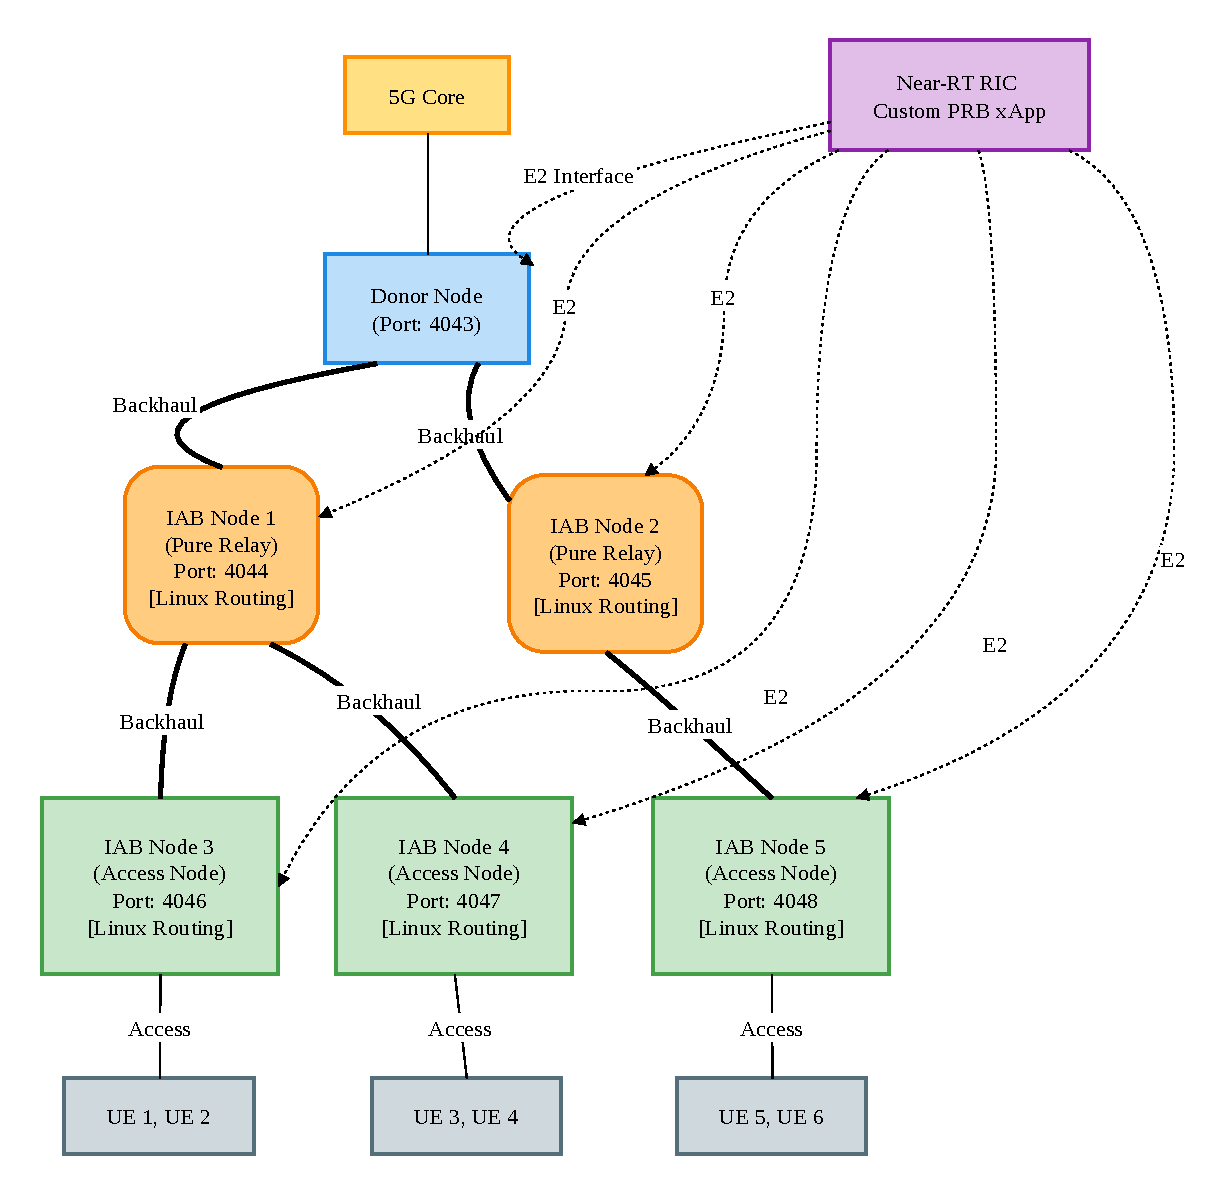
\includegraphics[width=\linewidth]{iab_architecture.pdf}
    \caption{The proposed tree-topology IAB architecture featuring Linux IP routing and xApp-based PRB allocation.}
    \label{fig:iab_arch}
\end{figure}

\subsection{Topology Overview}
Figure \ref{fig:iab_arch} illustrates the tree topology used in this work. The donor node connects the 5G Core to downstream IAB nodes. Intermediate nodes are organized into a relay layer that extends coverage hop by hop, while the leaf-side IAB nodes simultaneously maintain backhaul connectivity and provide access service to UEs. This separation of pure relay and access-capable relay roles makes it possible to study where bottlenecks emerge when traffic traverses multiple wireless hops.

\subsection{Infrastructure and Software Stack}
Each node is deployed on a high-performance Ubuntu 22.04 host equipped with a PREEMPT\_RT low-latency kernel to preserve the timing determinism required by the OAI baseband stack. USRP B210 and N310 devices are used as the SDR front-end, and OAI provides the 5G NR protocol implementation for the donor, IAB, and UE functions. In our implementation, the IAB-related functions are containerized and orchestrated with Docker Compose, which simplifies software management and improves experimental reproducibility across hosts while preserving access to the required radio and networking interfaces. This combination allows us to evaluate the PRB allocation strategy under realistic radio and host-processing constraints rather than relying only on software simulation.

From a deployment viewpoint, the testbed is split into a server-side Docker Compose stack and a client-side Docker Compose stack. The server-side stack hosts the O-RAN control components and core infrastructure, including FlexRIC, monitoring and control xApps, auxiliary inference services, MongoDB, the 5G Core, the donor node, and upper-layer IAB nodes. The client-side stack hosts the downstream access IAB nodes and the UE containers attached to them. This split deployment reflects the actual distribution of computation and radio functions across multiple PCs while keeping the full experiment manageable through declarative container orchestration.

\subsection{BAP-less Implementation via Linux Routing}
According to 3GPP specifications, IAB nodes rely on the BAP layer to manage routing and bearer mapping across multi-hop topologies. However, in open-source SDR deployments, a complete BAP implementation introduces additional encapsulation complexity, software overhead, and debugging difficulty.

To overcome this issue, we adopt a BAP-less architecture. In each IAB node, the IAB Mobile Termination (MT) for upstream connectivity and the IAB Distributed Unit (DU) for downstream service are co-located on the same physical host and deployed as containerized Docker Compose services. Instead of forwarding packets through a dedicated BAP layer, we use the native Linux kernel networking stack.

The OAI MT establishes a Protocol Data Unit (PDU) session toward the 5G Core through the donor node and creates a virtual interface such as \texttt{oaitun\_ue1}. Meanwhile, the OAI DU maintains the tunnel and radio interfaces needed to serve downstream UEs. By enabling \texttt{net.ipv4.ip\_forward=1}, configuring static routes, and applying \texttt{iptables} NAT rules when needed, packets can be transferred directly at the IP layer from the MT-facing interface to the DU-facing interface, even when the corresponding OAI functions are running inside containerized Docker Compose services with appropriately mapped network namespaces and interfaces. In this way, the node bypasses Layer-2 BAP encapsulation and performs lightweight multi-hop forwarding through Linux routing.

The container networks are also designed to match the experimental roles of the nodes. For example, the server-side stack uses a macvlan-based public network for inter-node signaling together with a bridge network for user-plane traffic toward the data network, whereas the client-side stack combines a macvlan segment for upstream IAB connectivity and an internal bridge network for local MT, DU, and UE interaction. In several control-plane services, host networking is used to simplify access to SCTP- and E2-related interfaces and to avoid unnecessary address translation between the containerized O-RAN functions and the host system.

\subsection{Near-RT RIC and xApp Integration}
For the control plane, we integrate FlexRIC as the near-RT RIC platform. The E2 interface is established between FlexRIC and the MAC entities of the donor DU and IAB DUs, enabling centralized observation and control over the radio resource state. The custom xApp periodically retrieves Buffer Status Reports (BSRs) and downlink scheduling statistics through the E2SM-MAC service model (SM ID 142), which exposes per-UE MAC-layer indicators from each DU. Based on the aggregated BH and AC buffer states, the xApp computes an updated PRB split and delivers the control decision via an E2 CONTROL message using the same E2SM-MAC service model's control procedure, allowing the MAC scheduler to enforce the new PRB quota without modifying the overall O-RAN control architecture.

In the current implementation, the near-RT RIC and xApps are launched in the server-side Compose stack together with supporting database and inference services. This arrangement is useful because it co-locates the closed-loop control applications with the main orchestration environment, while the client-side Compose stack focuses on hosting the downstream IAB nodes and UEs that generate the radio measurements and traffic loads consumed by the control loop.

The xApps were deployed as separate containers and attached to the same Docker Compose-managed control environment as FlexRIC.

% --- Section V: Allocation Schemes ---
\section{xApp-based PRB Allocation Schemes}
We evaluate the system using different PRB allocation strategies, including fixed-ratio allocation, adaptive xApp control, and the default PF scheduler.

\subsection{Scheme A: Fixed-Ratio Allocation}
In the first class of methods, the total PRBs are partitioned using a fixed ratio between backhaul and access, such as 50/50, 30/70, or 10/90. These settings serve as controlled experimental points for observing how resource imbalance shifts the bottleneck across the multi-hop path. A balanced split may not always be best: under some traffic patterns it can under-provision backhaul, whereas under others it can leave access capacity underutilized.

\subsection{Scheme B: Dynamic Traffic-Aware Allocation}
To complement the fixed-ratio settings, we implemented a dynamic allocation algorithm. The xApp continually monitors the transmission buffers. If the buffer of the Donor DU (backhaul link) exceeds a predefined threshold while the IAB DU (access link) buffer is nearly empty, the xApp reallocates a larger percentage of PRBs to the backhaul link, and vice versa. The logic is summarized in Algorithm \ref{alg:dynamic}. This scheme is included as another comparison point; its purpose is to examine whether queue-aware control produces a different operating point from fixed ratios and from the default proportional fair (PF) scheduler.

\subsection{Reference Scheduler: Default PF Scheduler}
In addition to the xApp-controlled policies, we use the default proportional fair (PF) scheduler in OAI as a reference case. The PF scheduler is not expected to be dominated by every handcrafted PRB split, especially when channel-aware fairness and instantaneous radio conditions strongly influence scheduling decisions. Therefore, the purpose of our evaluation is to compare behaviors and trade-offs, not to claim that the xApp-based methods universally outperform PF in throughput.

\begin{algorithm}[htbp]
\caption{Dynamic Traffic-Aware PRB Allocation}
\label{alg:dynamic}
\begin{algorithmic}[1]
\REQUIRE $BSR_{BH}$ (Backhaul Buffer), $BSR_{AC}$ (Access Buffer)
\REQUIRE $PRB_{total}$, Threshold $\tau$
\STATE Initialize $PRB_{BH} \gets PRB_{total}/2$, $PRB_{AC} \gets PRB_{total}/2$
\WHILE{E2 connection is active}
    \STATE Receive E2 Indication message
    \STATE Update $BSR_{BH}$ and $BSR_{AC}$
    \STATE Calculate load ratio: $\rho = \frac{BSR_{BH}}{BSR_{BH} + BSR_{AC} + \epsilon}$
    \IF{$|\rho - 0.5| > \tau$}
        \STATE $PRB_{BH} \gets \lfloor \rho \times PRB_{total} \rfloor$
        \STATE $PRB_{AC} \gets PRB_{total} - PRB_{BH}$
        \STATE Encode E2 Control message with new allocation
        \STATE Send E2 CONTROL to all subscribed DUs
    \ENDIF
    \STATE Wait for next monitoring interval $T_m$
\ENDWHILE
\end{algorithmic}
\end{algorithm}

% --- Section VI: Experimental Results ---
\section{Experimental Setup and Results}
This section details the empirical evaluation of the testbed.

\subsection{Setup Parameters}
The testbed components are deployed across multiple high-performance PCs running Ubuntu 22.04 with a PREEMPT\_RT low-latency kernel to ensure strict timing synchronization for the baseband processing. Table \ref{tab:parameters} lists the core parameters. Each policy was evaluated in a single continuous run of the six-epoch sequence (total $195$ s per policy). Throughput was measured using \texttt{iperf3} UDP in reverse mode (\texttt{-R}), with six UEs transmitting simultaneously, each connected to its own server port ($5201$--$5206$) on the \texttt{ext-dn} container. End-to-end latency was measured by \texttt{ping} with $1025$ probes per UE at $0.2$ s intervals ($-i\ 0.2$), spanning the full measurement window. No packet-loss filtering was applied; all RTT samples are included in the reported statistics.

\begin{table}[htbp]
\caption{Testbed Experimental Parameters}
\centering
\begin{tabular}{ll}
\toprule
\textbf{Parameter} & \textbf{Value} \\
\midrule
Operating System & Ubuntu 22.04 (Low-latency Kernel) \\
Deployment Method & Docker Compose-based multi-host deployment \\
Deployment Split & Server-side and client-side stacks \\
CPU Governor & Performance Mode \\
SDR Hardware & USRP B210 / N310 \\
Center Frequency & 3.5 GHz (Band n78) \\
Channel Bandwidth & 40 MHz \\
Subcarrier Spacing & 30 kHz \\
Software Stack & OpenAirInterface (OAI) + Docker Compose \\
RIC Framework & FlexRIC \\
Total PRBs & 106 \\
\bottomrule
\end{tabular}
\label{tab:parameters}
\end{table}

\subsection{Throughput Analysis}
We generated UDP traffic using \texttt{iperf3} to stress the multi-hop path under a reproducible six-epoch load sequence. Table~\ref{tab:traffic} summarizes the per-epoch settings. Each epoch lasts 30 seconds, and the same sequence is applied identically to all five policies to ensure a fair comparison.

\begin{table}[htbp]
\caption{Six-Epoch Traffic Sequence (6 UEs, Downlink)}
\centering
\begin{tabular}{llcc}
\toprule
\textbf{Ep.} & \textbf{Profile} & \textbf{UE\,1--4 (Mbps)} & \textbf{UE\,5--6 (Mbps)} \\
\midrule
1 & Balanced  & 5  & 5  \\
2 & BH-heavy  & 10 & 2  \\
3 & AC-heavy  & 2  & 10 \\
4 & Mixed     & 8/2 (alt.) & 6/3 \\
5 & Overload  & 8  & 8  \\
6 & Recovery  & 5  & 5  \\
\bottomrule
\end{tabular}
\label{tab:traffic}
\end{table}

Under this load sequence, the aggregate throughput (averaged across all six epochs) was: 50/50 = $25.80$ Mbps, 30/70 = $28.91$ Mbps, 10/90 = $29.71$ Mbps, adaptive = $29.85$ Mbps, and PF = $29.52$ Mbps. The small aggregate gap between the adaptive policy and PF ($0.33$ Mbps) reflects epoch-level variation: in the BH-heavy epoch, PF achieves $28.4$ Mbps while the adaptive xApp achieves $28.2$ Mbps; in the AC-heavy epoch, adaptive reaches $28.0$ Mbps while fixed-50/50 drops to $20.9$ Mbps. The per-epoch results reveal policy-dependent bottlenecks: in the BH-heavy epoch (Epoch~2), PF slightly outperforms the adaptive policy ($28.4$ vs.\ $28.2$ Mbps), while in the AC-heavy epoch (Epoch~3) the gap between fixed-50/50 and the adaptive policy widens to $7.1$ Mbps ($20.9$ vs.\ $28.0$ Mbps). The consistent aggregate advantage of more access-oriented splits confirms that the bottleneck under the evaluated downlink profile resides primarily at the access DU, not the relay backhaul link.

Under the evaluated downlink traffic profile, allocating more PRBs to the access links allows access DUs to serve UEs more efficiently, while backhaul relay links operate within their reduced quotas without becoming the dominant bottleneck. This conclusion is specific to the tested scenario; a predominantly uplink or relay-saturated workload would likely shift the bottleneck to the backhaul and favor a higher BH ratio. As a result, more access-oriented splits (30/70 and 10/90) outperform the balanced split (50/50) in aggregate throughput. The adaptive xApp, by dynamically adjusting the BH/AC ratio in response to buffer state measurements, achieves the highest aggregate throughput among all evaluated methods.

Importantly, the purpose of this comparison is not to claim that a handcrafted policy always exceeds PF. Instead, the measured values reveal how each method behaves under the same traffic condition. The PF scheduler achieves $29.52$ Mbps---slightly below the adaptive policy but above the balanced fixed split---demonstrating that the default scheduler finds a competitive operating point through its channel-aware fairness mechanism.

\begin{figure}[htbp]
    \centering
    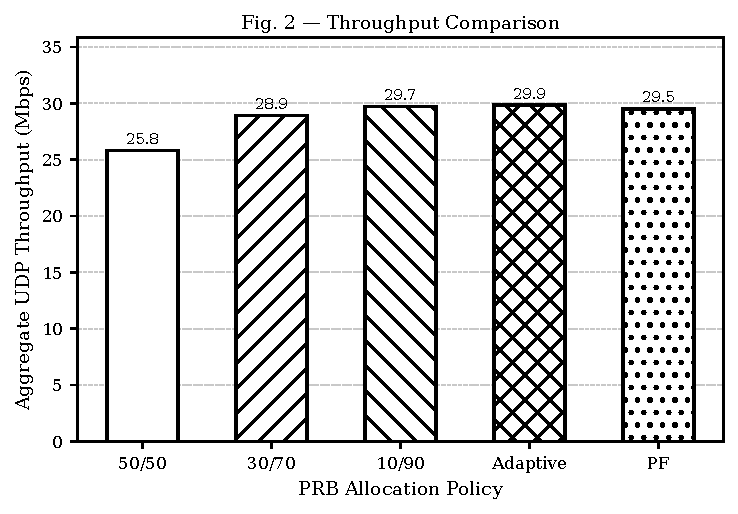
\includegraphics[width=\linewidth]{fig2_throughput.pdf}
    \caption{Throughput comparison among fixed-ratio allocation, adaptive xApp control, and the default PF scheduler under varying network loads.}
    \label{fig:throughput}
\end{figure}

\subsection{End-to-End Latency}
Latency is a critical metric for 5G services. The BAP-less Linux routing inherently introduces some processing delay at the kernel level. However, poor PRB allocation exacerbates this by causing packets to wait in the MAC layer queues. 

\begin{figure}[htbp]
    \centering
    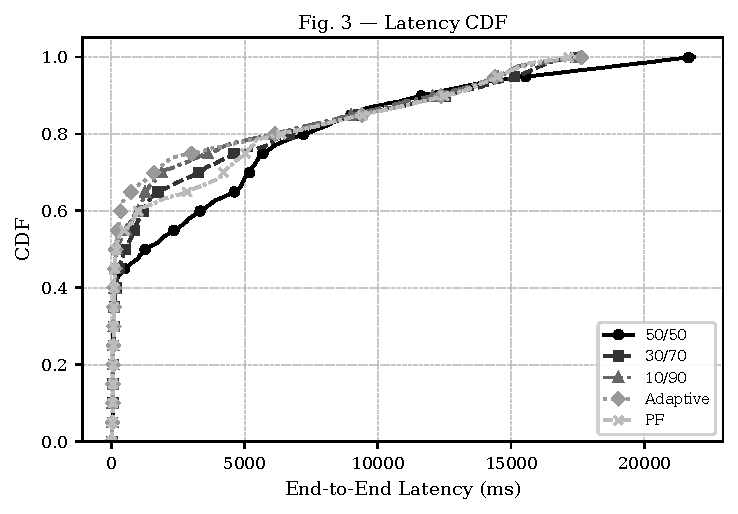
\includegraphics[width=\linewidth]{fig3_latency_cdf.pdf}
    \caption{Cumulative Distribution Function (CDF) of end-to-end latency for fixed-ratio allocation, adaptive xApp control, and the default PF scheduler.}
    \label{fig:latency}
\end{figure}

Figure \ref{fig:latency} illustrates the Cumulative Distribution Function (CDF) of the packet latency measured by ping RTT across all six epochs. The ping probes run continuously for the full $195$ s measurement window, capturing RTT samples under all traffic conditions including the AC-heavy epoch (Epoch~3), the overload epoch (Epoch~5, all UEs at $8$ Mbps), and the recovery epoch (Epoch~6). The absolute latency values are elevated relative to production deployments and are not intended to represent production-grade performance. This is expected in an RF-simulated multi-hop stack, where software-based baseband processing, Docker container scheduling, and multi-layer Linux IP forwarding each introduce queuing overhead that accumulates across relay hops. The measured RTT distribution also includes samples from the overload epoch (Epoch~5), during which all six UEs simultaneously inject 8~Mbps, contributing the highest-latency tail. Nonetheless, the relative ordering among policies is stable across epochs and reflects the underlying PRB allocation effects on queue depth.

The mean latency values of the 50/50 split, the 30/70 split, the 10/90 split, the adaptive xApp, and PF were $3890$ ms, $3294$ ms, $2976$ ms, $2897$ ms, and $3288$ ms, respectively, while the corresponding 95th-percentile latencies were $15694$ ms, $15160$ ms, $14564$ ms, $14439$ ms, and $14529$ ms. These results show a consistent trend: allocating more PRBs to the access links reduces end-to-end queuing delay, because access DUs can drain their downlink queues more quickly. The adaptive xApp achieves the lowest mean latency ($2897$ ms) and the lowest 95th-percentile latency ($14439$ ms) among all evaluated methods, indicating that its dynamic buffer-aware reallocation effectively reduces queue buildup across the diverse epoch conditions. The 50/50 split, which reserves a larger share for backhaul, exhibits the highest mean latency ($3890$ ms) and the highest 95th-percentile latency ($15694$ ms), consistent with a scenario where access resources are under-provisioned. The PF scheduler achieves a mean latency of $3288$ ms and a 95th-percentile of $14529$ ms, positioned between the more access-oriented fixed strategies and the balanced split. These results suggest that no single allocation rule is universally optimal across all traffic conditions, and that the throughput-latency trade-off is shaped by where in the relay chain the dominant bottleneck resides.

\subsection{System Resource Utilization}
Operating OAI alongside a near-RT RIC requires substantial computational power. We monitored the CPU utilization of the two relay DU containers (\texttt{rfsim5g-iab-du} and \texttt{rfsim5g-iab-du-2}) on PC1 via \texttt{docker stats} sampled every 5~s throughout each policy run. Table~\ref{tab:cpu} reports the per-container mean CPU averaged across both relay DUs and all samples within each run. The dominant cost in all cases is the OAI baseband processing thread, which consistently occupies approximately $48$--$51$\% of a single CPU core regardless of the PRB policy applied. Compared with the fixed-ratio baseline (fixed-50/50: $48.8$\%), the adaptive xApp policy incurred a per-container mean of $49.7$\%---a difference of less than $1$\%, well within the stated threshold of $3$\%. This confirms that the xApp control loop, which runs at the near-RT RIC and communicates via E2 over SCTP, does not measurably starve the baseband processing threads.

\begin{table}[htbp]
\caption{Mean Relay DU CPU Utilization per Policy}
\centering
\begin{tabular}{lcc}
\toprule
\textbf{Policy} & \textbf{Mean CPU (\%)} & \textbf{$\Delta$ vs.\ Fixed-50/50} \\
\midrule
Fixed 50/50 & 48.8 & --- \\
Fixed 30/70 & 47.5 & $-1.3$ \\
Fixed 10/90 & 50.0 & $+1.2$ \\
Adaptive    & 49.7 & $+0.9$ \\
PF (no xApp)& 51.4 & $+2.6$ \\
\bottomrule
\end{tabular}
\label{tab:cpu}
\end{table}

% --- Section VII: Conclusion ---
\section{Conclusion}
In this paper, we presented a practical multi-hop O-RAN IAB testbed and demonstrated that a BAP-less forwarding design based on Linux IP routing is feasible for SDR-based relay deployment. We further integrated a near-RT RIC and a custom xApp to implement multiple PRB allocation methods between backhaul and access links. The resulting platform enables direct experimental comparison among fixed-ratio configurations, an adaptive xApp policy, and the default PF scheduler in a real implementation environment. Our results show that these allocation methods exhibit different throughput-latency trade-offs, highlighting that the value of the proposed platform lies in empirically characterizing such behaviors rather than asserting that any single handcrafted policy consistently outperforms PF.

As future work, we plan to extend this framework toward hierarchical O-RAN control. In particular, a non-real-time RIC can host an rApp based on deep reinforcement learning (DRL) to learn long-term traffic patterns, topology states, and performance trends from historical observations. The learned policy can then be transferred from the non-RT RIC to the near-RT RIC, where an xApp executes the policy through near-real-time PRB control over E2-connected nodes. Such collaboration between the non-RT RIC and near-RT RIC is expected to better align with the O-RAN architecture and to support more adaptive throughput-latency trade-offs under diverse traffic conditions.

% --- Acknowledgment ---
\section*{Acknowledgment}
The authors thank the open-source communities of OpenAirInterface and FlexRIC for their foundational contributions.

% --- References ---
\bibliographystyle{IEEEtran}
\bibliography{references}

\end{document}